It is previously mentioned that activity represents a screen with a committed user interface. Nevertheless, an activity might also include one or more fragments. In the Android world, the term “fragment” is used to picture a behavior or a part of a user interface in an activity. Although fragments are not one of the main Android application components that were previously mentioned in this study, they are worth discussing briefly due to the fact that fragments have their own lifecycle and they are highly connected to the activities in that sense. The figure below is an illustration of the fragment lifecycle and it presents the fragment lifecycle methods.
\begin{figure}[ht!]
    \centering
    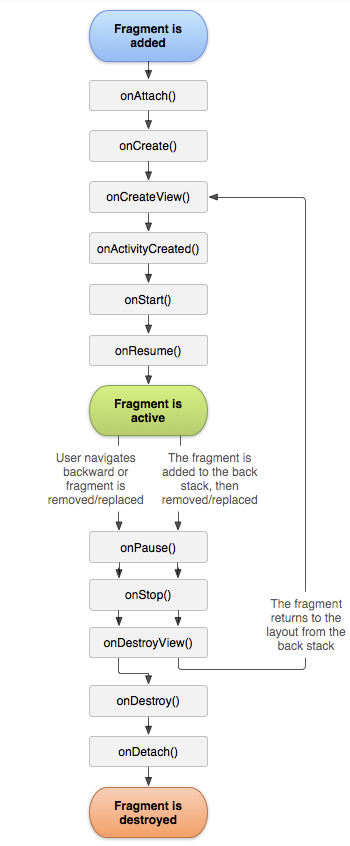
\includegraphics[scale=0.4]{figures/fragment_life_cycle.png}
    \caption{Android fragment lifecycle \protect\footnotemark}
    \label{fig:android_fragment_life_cycle}
\end{figure}
\footnotetext{\url{https://developer.android.com/guide/fragments/lifecycle}}
\FloatBarrier
A fragment can be considered as a modular part of an activity. Fragments can be combined in an activity to build multi-window user interfaces. Fragments have their own lifecycle and input events. Unlike activities, fragments are reusable and reuse of a fragment in multiple activities is possible. Fragments cannot exist on their own. Every fragment is hosted by an activity. That makes the lifecycle of a fragment directly related to the lifecycle of the host activity that the fragment was created in. 

Fragments are represented by the “Fragment” class of the Android Software Development Kit. In order to create a fragment, a class must inherit the Fragment class or existing subclasses of the Fragment class. It was already indicated that, though fragments have a lifecycle that is tightly coupled with their host activity lifecycle, they have their own lifecycle which is different than the activities’ lifecycle. Thus fragments have their own lifecycle callback methods. The study already aforementioned that why having good knowledge regarding activity lifecycle callback methods is important. The importance of the fragment lifecycle callback methods is no different as well. Proper understanding of fragment lifecycle callback methods helps developers to know when to add/release these non-UI related components to fragments when building maintainable Android applications based on fragments.

In the same way as activity lifecycle, the fragment lifecycle exists in three states as well and these states are "resumed", "paused", and "stopped". Transitions between these states are managed by the system through the callback methods presented in the figure above. Detailed explanations of the importance of the fragment lifecycle methods and their functionality can be found in the Android developer guidelines. 